\documentclass[10pt]{article}
\usepackage[margin=0.55in]{geometry}
\usepackage{times,xcolor,titlesec,graphicx,hyperref}
\definecolor{maroon}{HTML}{500000}
\titleformat{\section}{\normalsize\bfseries\color{maroon}}{}{0pt}{}
\titlespacing{\section}{0pt}{6pt}{2pt}
\setlength{\parindent}{0pt}\setlength{\parskip}{3pt}
\hypersetup{colorlinks=true,linkcolor=maroon,urlcolor=maroon}
\pagestyle{empty}
\begin{document}
{\color{maroon}\rule{\linewidth}{4pt}}
{\bfseries\large\color{maroon} UI checkpoint: Aggie Course Scout}\hfill Carlos Luna-Pena, CSCE 470
{\color{maroon}\rule{\linewidth}{1pt}}

\section*{Design direction}
Maroon and cream, drawn from TAMU print materials but kept quiet. Results read like catalog cards: serif title, small metadata, highlighted snippet, rank score. The search syntax is visible under the box instead of hidden in a help page. Facets sit to the left on desktop and stack above results on mobile. The detail drawer shows the full description, prerequisites, and the term-level ranking table.

\section*{Desktop results}
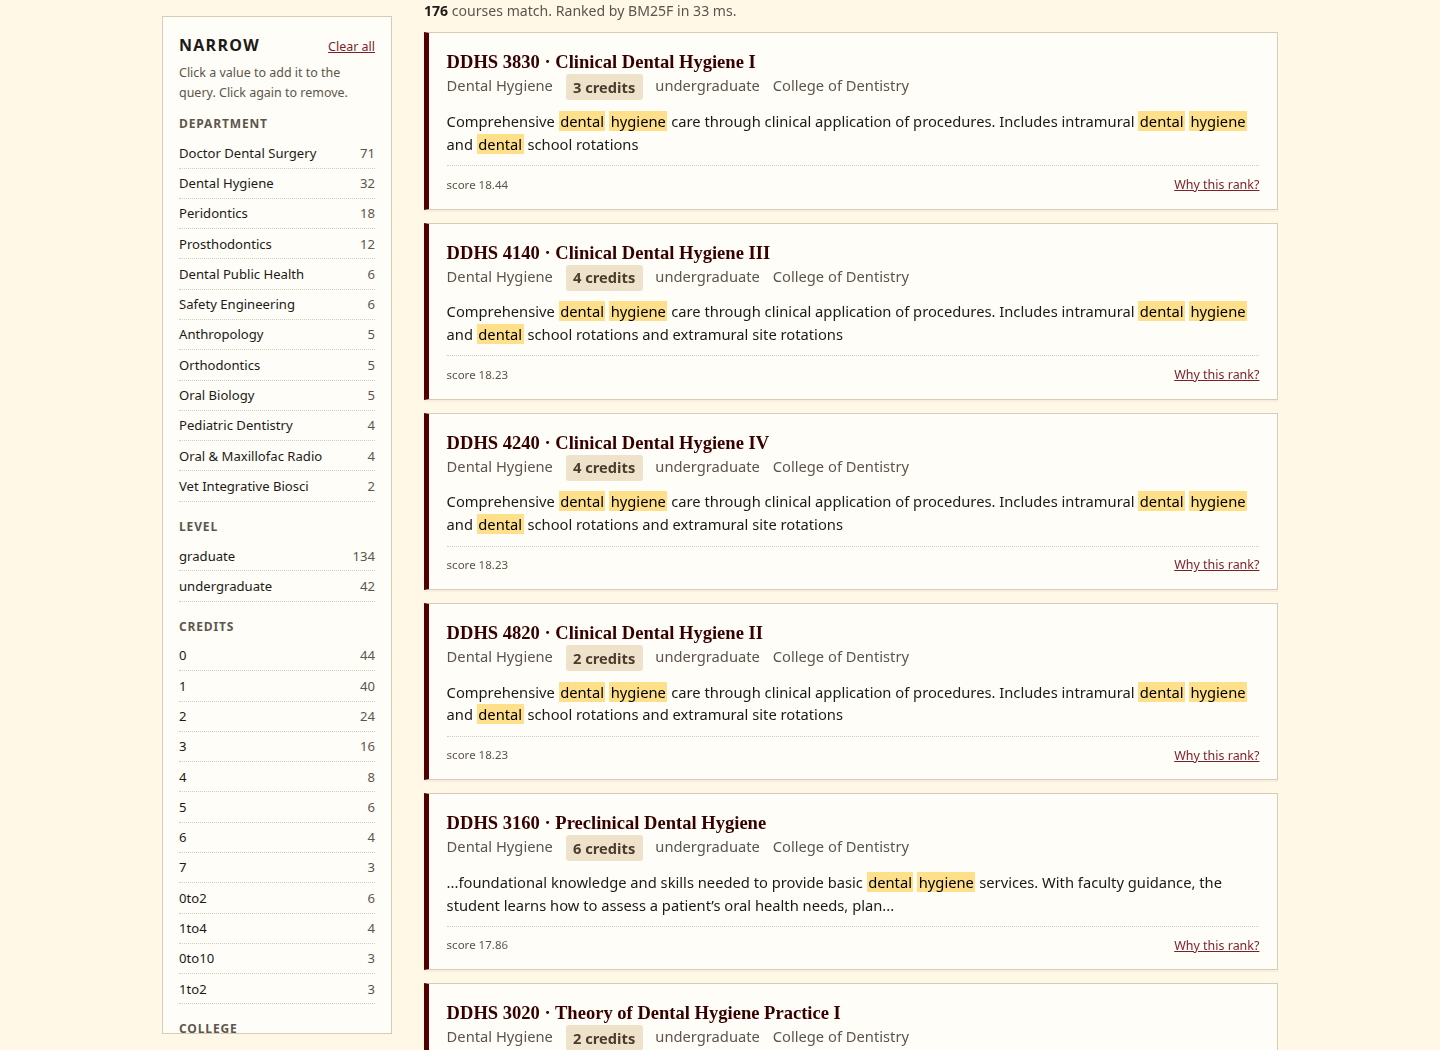
\includegraphics[width=\linewidth]{../web/assets/screenshots/desktop-results.png}
\smallskip
{\footnotesize The query \texttt{dental hygiene} returns 176 records. Clinical Dental Hygiene I is first, and the snippet marks both query terms. Department facets show names, not codes. The facet counts come from the filtered result set, not the whole index.}

\newpage
\section*{Mobile layout and detail panel}
\begin{minipage}[t]{0.36\linewidth}
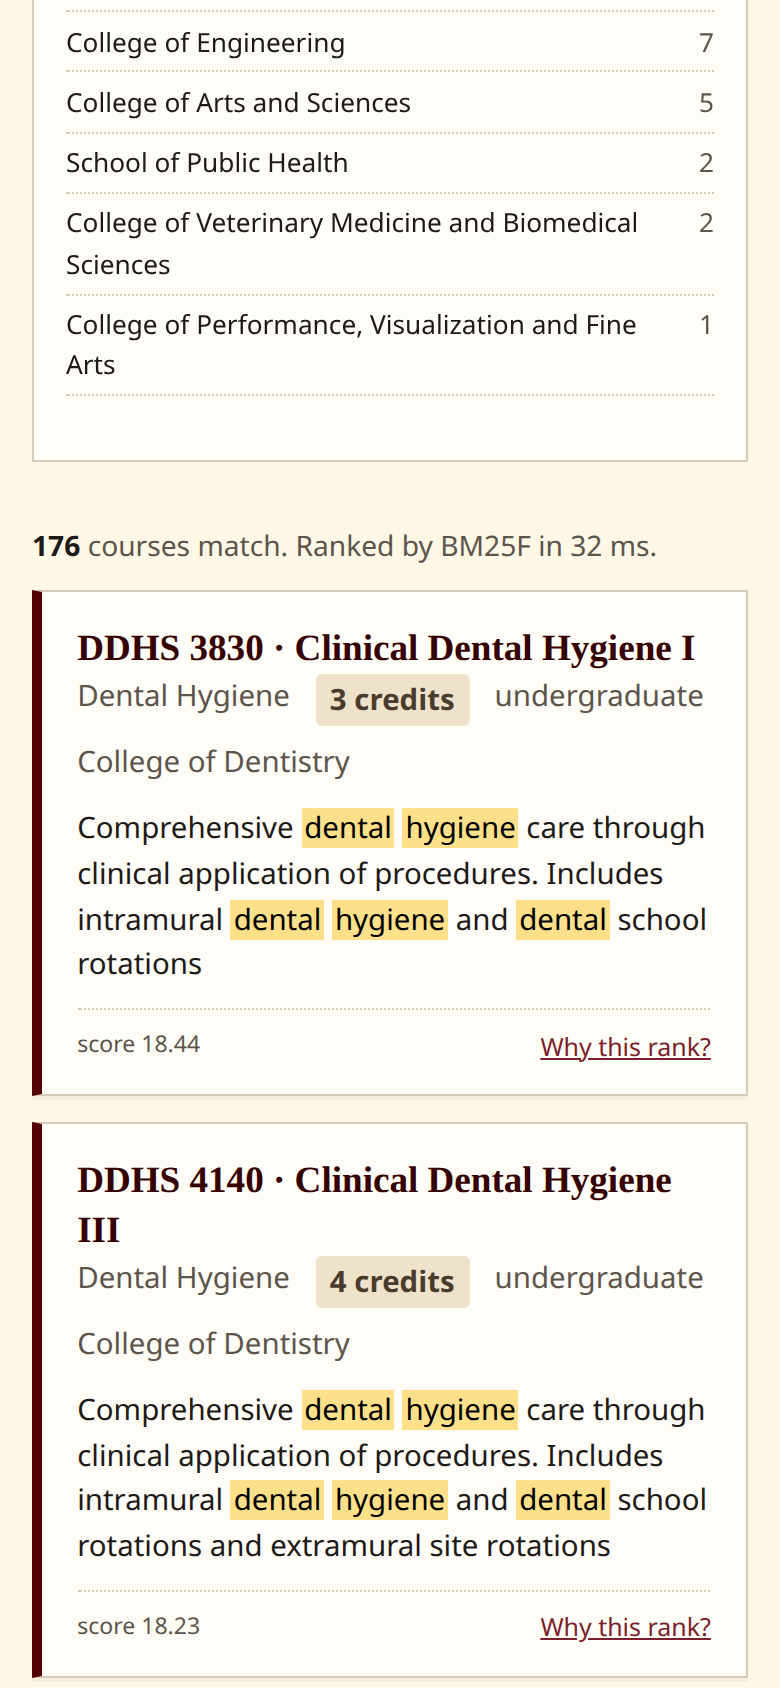
\includegraphics[width=\linewidth]{../web/assets/screenshots/mobile-results.png}
\end{minipage}\hfill
\begin{minipage}[t]{0.60\linewidth}
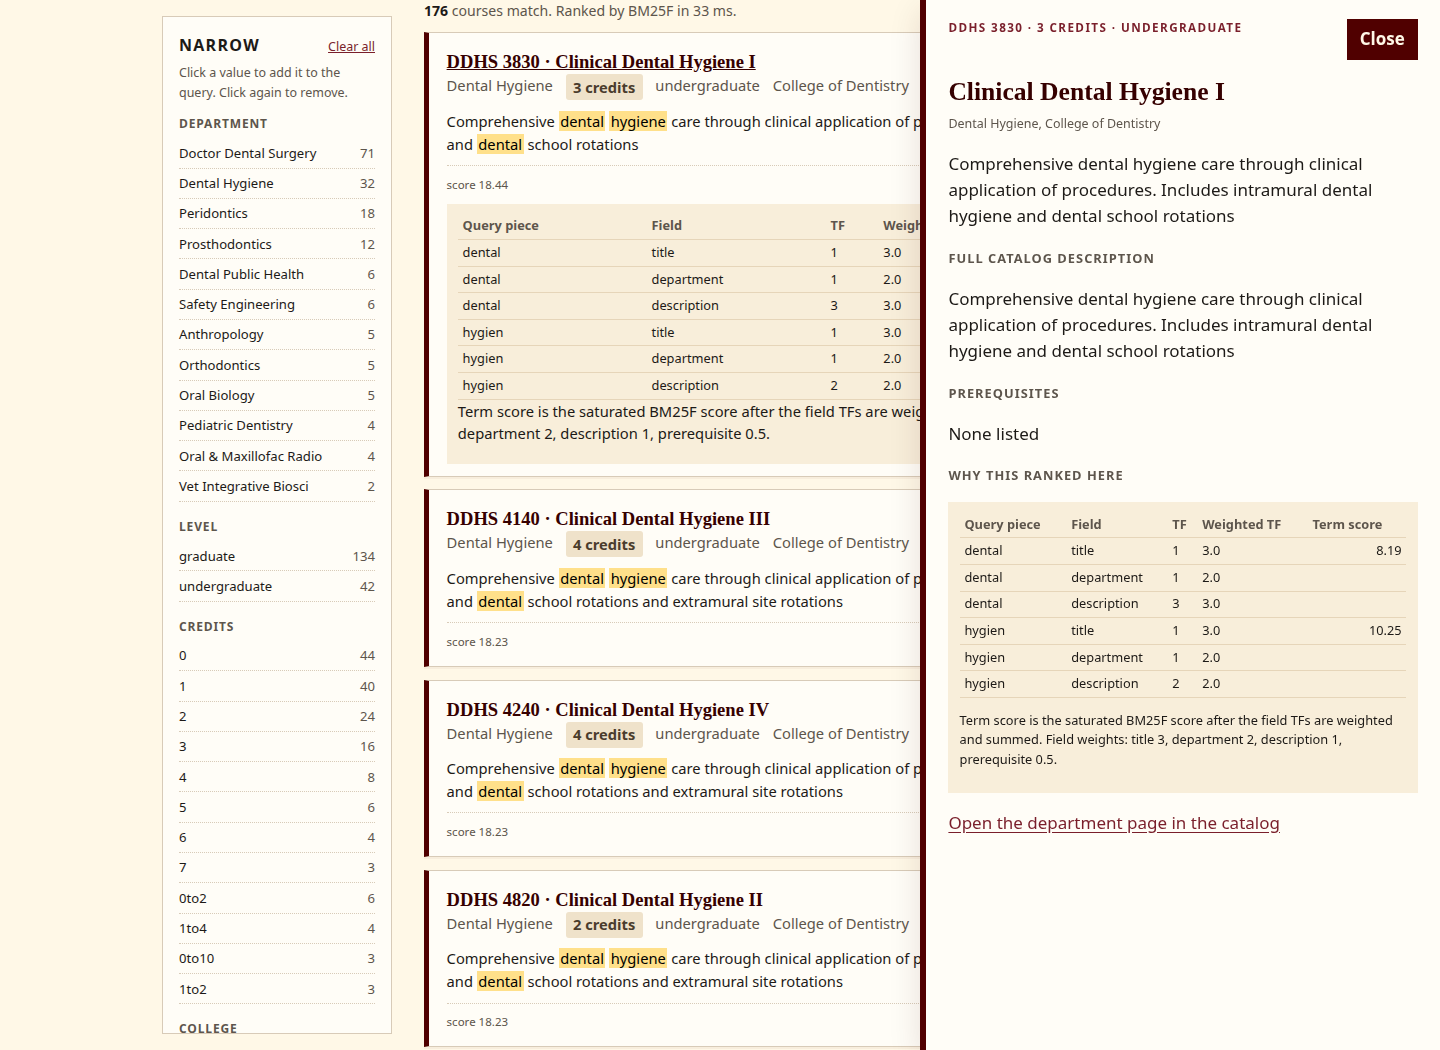
\includegraphics[width=\linewidth]{../web/assets/screenshots/detail-panel.png}
\end{minipage}

\smallskip
{\footnotesize Left: 390 px viewport, one column, no horizontal scroll. Right: detail panel with the department name, full catalog text, prerequisites, and the why-this-ranked table.}

\section*{States and accessibility}
There are explicit loading, empty, and index-error states. The loading state names the index size. The empty state suggests removing a filter or fixing spelling. The status region is an ARIA live region. Markup uses a skip link, real buttons, visible focus rings, 4.5:1 or better body contrast, and a reduced-motion media query. Escape closes the detail panel and slash focuses search.

\section*{What changed after testing}
The first detail view looked up the description by the result's position in the ranked list instead of its document id, so it could show the wrong course. The browser test caught it. The why table also repeated one term score on every field row; it now shows weighted TF per field and the term score once. The mobile facet column originally stayed sticky and ate the viewport, so it was set to static below 780 px.

\section*{Known rough edges}
The result cards still show raw credit strings such as \texttt{0to4}. Long department names wrap awkwardly at 390 px. The detail drawer covers the results with no backdrop on mobile, so the context behind it is only partly visible.

\end{document}
